\documentclass[letterpaper,12pt,fleqn]{article}
\usepackage{matharticle}
\usetikzlibrary{decorations.pathmorphing}
\pagestyle{empty}
\newcommand{\e}{\epsilon}
\renewcommand{\O}{\Omega}
\newcommand{\uc}{\rightrightarrows}
\newcommand{\norm}[2]{\left\|#1\right\|_{#2}}
\newcommand{\inorm}[1]{\norm{#1}{\infty}}
\newcommand{\cf}{\mathcal{C}}
\begin{document}
\section*{Uniform Convergence}

\begin{definition}[Uniform Convergence]
  Let $f_n$ be a sequence of functions. To say that $f_n$
  \emph{converges uniformly} to $f$ over an interval $\O$, denoted $f_n\uc f$,
  means:
  \[\forall\,\e>0,\exists\,N(\e)>0,\forall\,x\in\O,
  n>N\implies\abs{f_n(x)-f(x)}<\e\]
\end{definition}

\begin{figure}[h]
  \centering
  \begin{tikzpicture}[scale=2]
    \draw (-0.5,0) -- (6,0);
    \draw (0,-0.5) -- (0,4);
    \draw [dashed] (1,-0.5) -- (1,4);
    \draw [dashed] (5,-0.5) -- (5,4);
    \node [below] at (3,0) {$\O$};
    \draw plot [smooth] coordinates {(1,1) (3,3) (4,2) (5,3)};
    \draw [decorate, decoration={zigzag, segment length=20mm, amplitude=5mm}]
    plot coordinates {(1.1,1) (3,3) (4,2) (5,3)};
    \draw [dashed] plot [smooth] coordinates {(1,1.5) (3,3.5) (4,2.5) (5,3.5)};
    \draw [dashed] plot [smooth] coordinates {(1,0.5) (3,2.5) (4,1.5) (5,2.5)};
    \node [above left] at (1,1) {$\e$};
    \node [below left] at (1,1) {$\e$};
    \node [above] at (3,3) {$f$};
    \node [below] at (3,2.9) {$f_n$};
  \end{tikzpicture}
\end{figure}

\begin{theorem}[Uniform Convergence Norm]
  Let $E$ be a function space and $(f_n)$ be a sequence of functions in $E$.
  \[f_n\uc f\iff\inorm{f_n-f}\to0\]
\end{theorem}

\begin{theproof}
  \listbreak
  \begin{eqnarray*}
    f_n\uc f &\iff& \forall\,\e>0,\exists\,N(\e)>0,\forall\,x,
    n>N\implies\abs{f_n(x)-f(x)}<\e \\
    &\iff& \forall\,\e>0,\exists\,N(\e)>0,\forall\,x,
    n>N\implies\max\{\abs{f_n(x)-f(x)}\}<\e \\
    &\iff& \forall\,\e>0,\exists\,N(\e)>0,\forall\,x,
    n>N\implies\inorm{f_n-f}<\e \\
    &\iff& \inorm{f_n-f}\to0
  \end{eqnarray*}
\end{theproof}

\newpage

But is there such a norm for pointwise convergence?

\begin{definition}[Pointwise Convergence]
  Let $f_n$ be a sequence of functions. To say that $f_n$
  \emph{converges pointwise} to $f$ over an interval $\O$, denoted $f_n\to f$,
  means:
  \[\forall\,x\in\O,\forall\,\e>0,\exists\,N(\e,x)>0,
  n>N\implies\abs{f_n(x)-f(x)}<\e\]
\end{definition}

Consider the following counterexample. Let $g_n(t)\in\cf[0,1]$ be defined by:

\bigskip

\begin{minipage}{3.5in}
  \[g_n(t)=\begin{cases}
  2^nt, & 0\le t\le2^{-n} \\
  2-2^nt, & 2^{-n}\le t\le2^{-(n-1)} \\
  0, & otherwise
  \end{cases}\]
\end{minipage}
\begin{minipage}{3in}
  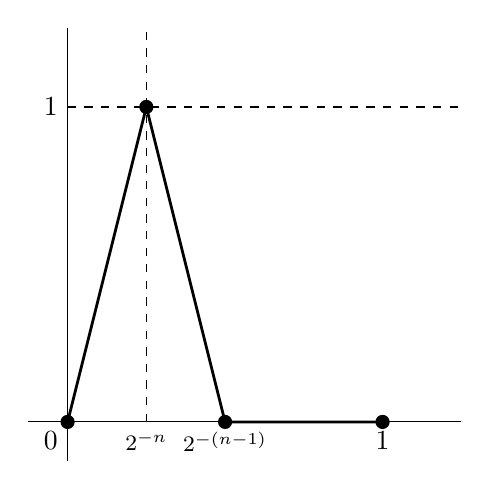
\begin{tikzpicture}
    \draw (-0.5,0) -- (5,0);
    \draw (0,-0.5) -- (0,5);
    \node [below left] at (0,0) {$0$};
    \node [below] at (4,0) {$1$};
    \node [left] at (0,4) {$1$};
    \draw [dashed] (0,4) -- (5,4);
    \draw [dashed] (1,0) -- (1,5);
    \draw [line width=1pt] (0,0) -- (1,4) -- (2,0) -- (4,0);
    \node [draw, circle, fill=black, scale=0.5] at (0,0) {};
    \node [draw, circle, fill=black, scale=0.5] at (1,4) {};
    \node [draw, circle, fill=black, scale=0.5] at (2,0) {};
    \node [draw, circle, fill=black, scale=0.5] at (4,0) {};
    \node [below] at (1,0) {\footnotesize$2^{-n}$};
    \node [below] at (2,0) {\footnotesize$2^{-(n-1)}$};
  \end{tikzpicture}
\end{minipage}

Assume $\norm{\cdot}{}$ is a norm on $\cf[0,1]$. By the properties of the norm,
$g_n$ is not the zero function and thus $\norm{g_n}{}\ne0$. Now, let:
\[f_n=\frac{g_n}{\norm{g_n}{}}\]
By the properties of the norm:
\[\norm{f_n}{}=\norm{\frac{g_n}{\norm{g_n}{}}}{}=
\frac{\norm{g_n}{}}{\norm{g_n}{}}=1\]
Assume $t\in[0,1]$. \\
Assume $\e>0$. \\
Note that as $t\to0$, $f_n(t)\to0$. \\
So AWLOG $t\ne0$. \\
There exists $N>0$ such that the non-zero part of $g_n$ is pushed to the left
of $t$ and thus $f_n(t)\to 0$. \\
Assume $n>N$: \\
\[\abs{f_n(t)}=\frac{g(t)}{\norm{g(t)}{}}=\frac{0}{\norm{g(t)}{}}=0<\e\]
Thus, $f_n\to0$ pointwise, but $\norm{f_n}{}\to1$.

Therefore, there is no suitable norm for pointwise convergence.
\end{document}
